
\documentclass{article}
\usepackage{graphicx}
\usepackage[top=3cm]{geometry}
\usepackage{tabularray}
\usepackage{afterpage}

\graphicspath{{./}}
\begin{document}

\begin{titlepage}
	\begin{center}
	\LARGE{ECE 8540 Analysis of Tracking System}\\
	\line(1,0){200}\\
	[5mm]
	\Large{Lab 2 report}\\
	\Large{Non-Linear Fitting}\\
	[150mm]
	\large{Harshal B. Varpe}\\
	Spetember 12, 2022
	\end{center}
\end{titlepage}
\begin{center}
\section{Introduction}\label{sec:intro}
\end{center}

Lab 2 focuses on calculating a nonlinear regression fit wihtout using any of the high-level functions that matlab or any other software package provides. The students are provided with 3 different datasets: A, B, and C. Each file has two columns x and y. We are to fit a fucntion of the form - 
Let us start with the derivation process of the non-linear regression.
For non-linear model fitting, we used the idea of root finding.We write an error function and find its minimum. The minimum could be found where the derivative of this function is zero. We are given that all the data sets follow the form of , where  is a non-linear unknown.
We can write the error function as follows -

\begin{equation}\label{eq1}
E = \sum_{i=1}^{N} (y_i-ln(ax_i)) ^2
\end{equation}

The partial derivative of the error function with respect to the unknown $a$:
\begin{equation}\label{eq2}
 \frac{\partial E}{\partial a} = \sum_{i=1}^N (-2)(y_i - ln(ax_i) * (\frac{1}{ax_i}) * x_i
\end{equation}
We can simplify the equation \ref{eq2} to the following form, since  is a constant with respect to $a$.
\begin{equation}\label{eq3}
\frac{\partial E}{\partial a} = \sum_{i=1}^{N}(y_i - ln(ax_i))(\frac{1}{a})
\end{equation}         
We wish to minimize the error, therefore we equate equation \ref{eq3} to 0.
 \begin{equation}\label{eq4}
\frac{\partial E}{\partial a} = \sum_{i=1}^{N}(y_i - ln(ax_i))(\frac{1}{a}) = 0
\end{equation}
We wish to use the root finding approach, which is an interative approach. In order to implement this iterative approach, we have a following equation:
\begin{equation}\label{eq5}
a_{n+1} = a_{n} - \frac{f(a_n)}{f'(a_n)}
\end{equation}
Let us assume -   
\begin{equation}\label{eq6}
f(a) = \sum_{i=1}^{N}(y_i - ln(ax_i))(\frac{1}{a})
\end{equation}
If we take a partial derivative of equation \ref{eq6}, we get :
\begin{equation}\label{eq7}
f'(a) = \sum_{i=1}^{N}(\frac{-1}{a^2})(y_i - ln(ax_i)+1)
\end{equation}

Now we substitute the equation \ref{eq6} and the equation \ref{eq7} in equation \ref{eq5} and solve for $a$. We make an initial guess for $a$ and then iterate untill the desired convergence is observed. \\
\newpage


\section{\centering Code and Result}\label{sec:code}

The following image shows  how the equations shown in section~\ref{sec:intro} are implemented in MATLAB. The inner loop with q as counter calculates the values for equations \ref{eq6} and \ref{eq7}. Based on these values, we calculate equation \ref{eq5}. Thus, we get a new guess. The outer loop with counter p initiates new calculations for the unknown with an updated guess. To avoid the infinite loop, in the case of divergence, we use a condition with variable$ p\_max$. If the diffrence between $(a_n)$ and $(a_{n+1})$ is greater then $p\_max$, then we break out of the for loop. The value of $p\_max$ is arbitrary. It is selected to suit the needs of the script. If the difference between  $(a_n)$ and $(a_{n+1})$ falls below $10^{-5}$, we stop the calculations as sufficient degree of accuracy is achieved. At the end we print out how many iteration it took to converge to the solution and the final value of the unknown.

\begin{figure}[ht]
	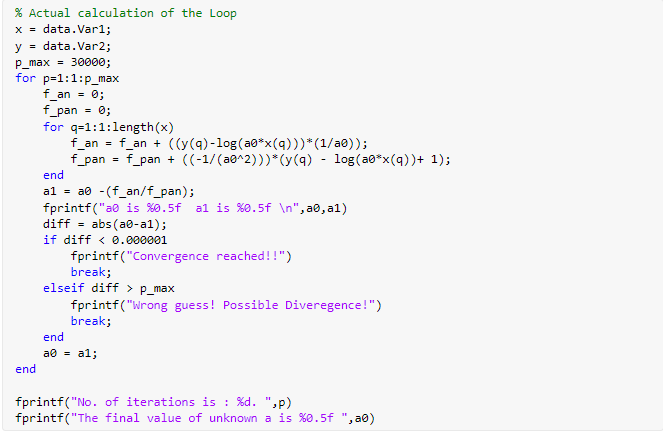
\includegraphics{Code.png}
	\caption{A snippet of the MATLAB script}
	\label{fig:snippet}
\end{figure}

We had three different datasets. For each of the dataset, five different initial guesses were considered. The purpose of selecting different initial guesses was to study the affect on converegence. Below are the three tables for each of the dataset containing initial guess, number of iteration for convergence ,and a convergence value.\\

In the table \ref{tab:dataA}, we can see the initial values chosen for the five iterations. As expected, as our initial guess gets closer to the answer or the approximate value of the unknown $a$, number of iteration required reduce. Although not shown here, if the initial guess differs from the final values of $a$ significantly, then converegence may not be reached. \\

\begin{table}[h!]
\centering
\begin{tblr}{| c | c | c |}
\hline
Initial Guess ($a$) &  Number of Iterations & Final value of $a$ \\
\hline
\hline
1 & 9 & 6.71136 \\
\hline
2&8&6.71136 \\
\hline
5&5&6.71136 \\
\hline
7&4&6.71136 \\
\hline
10&8&6.71136 \\
\hline
\end{tblr}
\caption{ Initial guesses for data set A}
\label{tab:dataA}
\end{table}

In the table \ref{tab:dataB}, we can see just like the Data set A, initial guess was 1. Since the initial guess was significantly lower than the final answer, it took 11 iterations to reach the final anwer.

\begin{table}[h!]
\centering
\begin{tblr}{| c | c | c |}
\hline
Initial Guess ($a$) &  Number of Iterations & Final value of $a$ \\
\hline
\hline
1 & 11 & 18.99612 \\
\hline
9&7&18.99612 \\
\hline
15&5&18.99612 \\
\hline
20&4&18.99612 \\
\hline
30&9&18.99612 \\
\hline
\end{tblr}
\caption{ Initial guesses for data set B}
\label{tab:dataB}
\end{table}

In the table \ref{tab:dataC}, we observe similar pattern. The closer our initial guess is to the final answer, the faster we converge to the solution. Initial guess of 1 did not work for this data set. As compared to the data set A and data set B, the initial guess had to be lowered to 0.2. It was observed that for the Initial guess value of 0.5, the algorithm failed to converge.\\

\begin{table}[ht!]
\centering
\begin{tblr}{| c | c | c |}
\hline
Initial Guess ($a$) &  Number of Iterations & Final value of $a$ \\
\hline
\hline
0.2 & 5 & 0.29000 \\
\hline
0.1&7&0.29000 \\
\hline
0.4&6&0.29000 \\
\hline
0.45&8&0.29000 \\
\hline
0.35&5&0.29000 \\
\hline
\end{tblr}
\caption{ Initial guesses for data set C}
\label{tab:dataC}
\end{table}


Below are the plots for each of the data sets.\\

\begin{figure}[!htb]
\centering
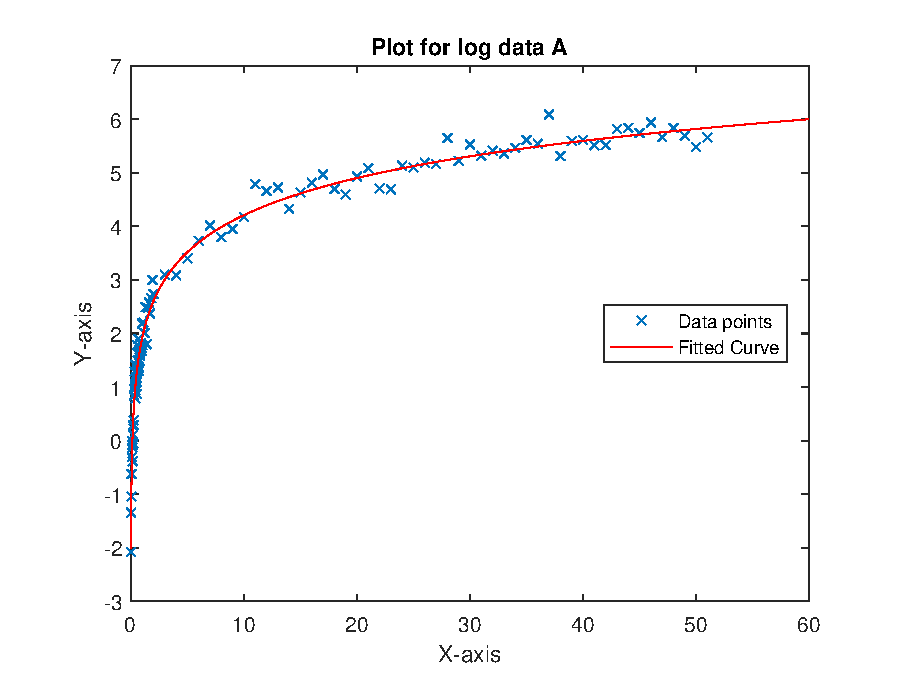
\includegraphics[scale=0.75]{Log_A.eps}
\label{plt:A}
\caption{Data points and fitted curve for Dataset A}
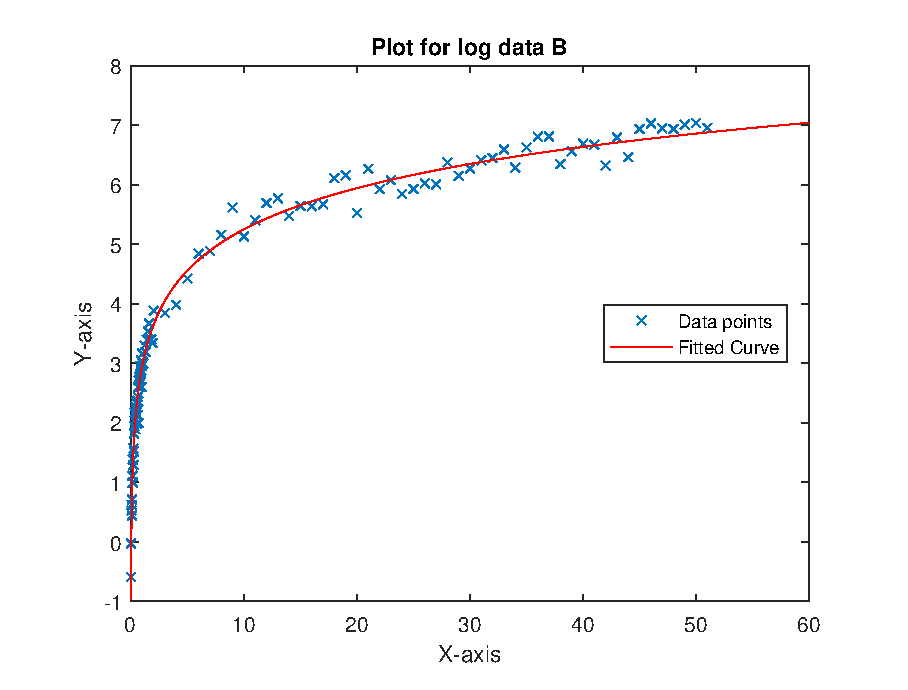
\includegraphics[scale=0.75]{Log_B.eps}
\label{plt:B}
\caption{Data points and fitted curve for Dataset B}
\end{figure}

\afterpage{
	\begin{figure}[!htb]
	\centering
	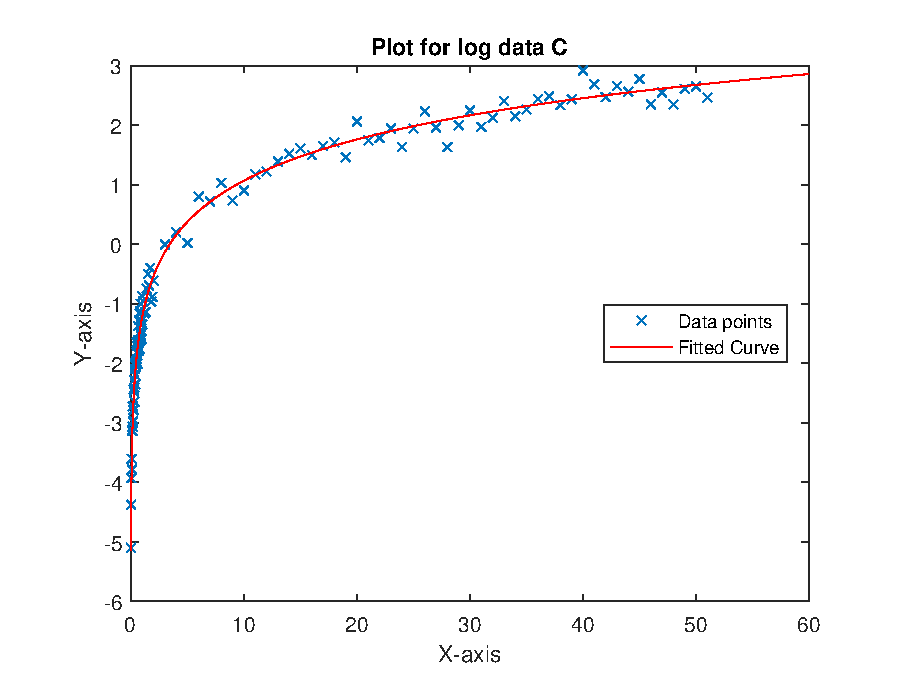
\includegraphics[scale=0.75]{Log_C.eps}
	\label{plt:C}
	\caption{Data points and fitted curve for Dataset C}
	\end{figure}
}
\clearpage

In summary, we can say that root finding techniques can be used for the purpose of non-linear curve fitting. One of the demerits of this technique is that the results are limited to initial guess. If the initial guess is far off from the solution, the convergence may not be reached leading to failure. However, within the certain limits for an initial guess, the technique is quite robust and consistent.


\end{document}